\begin{frame}{Historique}
	\begin{itemize}
		\item \textbf{1943 :} Le neurone formel \cite{McCulloch43}
		\newline Une représentation mathématique d’un neurone biologique.
		\item \textbf{1949 :} Loi d'adaptation \cite{Hebb49}
		\item \textbf{1958 :} Le perceptron \cite{Rosenblatt58}
		\item \textbf{1986 :} Le réseau récurrent de Jordan et Elman \cite{Jordan86}
	\end{itemize}
\end{frame}

\begin{frame}{Le neurone formel}
    
    \begin{columns}
        \begin{column}{.55\textwidth}
            \begin{figure}
                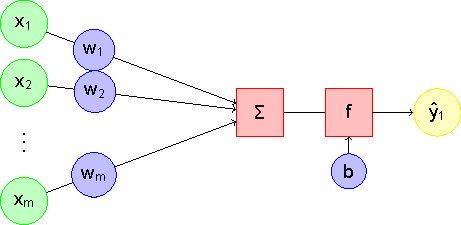
\includegraphics[height=.75\textheight,width=\textwidth,keepaspectratio]{images/neurone}
                \caption{Le neurone formel {\scriptsize\it -- Source : Cours R. \textsc{Hérault} \& P. \textsc{Leray}}}
            \end{figure}
        \end{column}
        \begin{column}{.45\textwidth}
    
            \begin{itemize}
                \item $x_i$ : entrées
                \item $w_i$ : poids
                \item $f$ : fonction d'activation
                \item $b$ : biais
                \item $\hat{y}$ : sortie du neurone
            \end{itemize}
        \end{column}
    \end{columns}
\end{frame}
